
\chapter{Capitulo 2}

Este capítulo fala de \gls{stemmer}s. Mas não esquecer os \Gls{lematizador}es

\section{Sub-capitulo 1}

O \acrfull{http} é um protocolo baseado em \acrshort{tcp}.

\section{Figuras}

Ao contrário do Word, o \LaTeX{} usa um mecanismo de colocação de figuras e tabelas em que estas
flutuam ao longo das páginas de acordo com a necessidade/disponibilidade em termo de espaço vertical.
Assim, não devem usar frases como ``na figura acima'', ou ``na figura abaixo'', mas fazer referências:
``tal como se pode observar na Figura~\ref{fig:1}.''

\begin{figure}[htb]
    \centering
    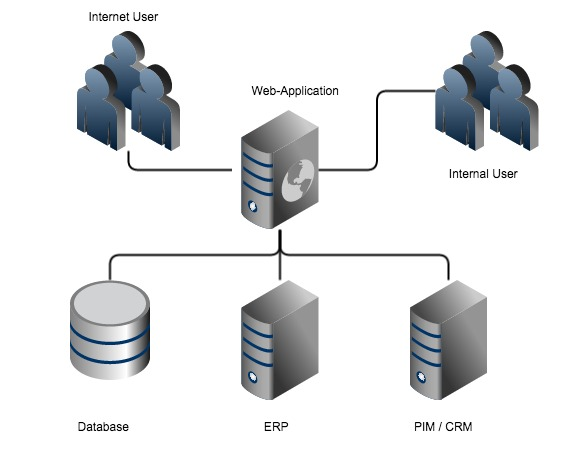
\includegraphics[width=0.8\linewidth]{images/sample}  % largura percentual 
    \caption{Esta é a legenda da figura}
    \label{fig:1}
\end{figure}

O mesmo acontece com as tabelas, como se pode ver na Tabela~\ref{tab:1}.

\begin{table}[htb]
    \centering
    \begin{tabular}{ccccc}
        \toprule
        \textbf{A} & \textbf{B} & \textbf{C} & \textbf{D} & \textbf{Total} \\
        \midrule
          1 & 2 & 3 & 4 & 10  \\
          2 & 3 & 4 & 5 & 14  \\
          3 & 4 & 5 & 6 & 18  \\
          4 & 5 & 6 & 7 & 22  \\
         \bottomrule
    \end{tabular}
    \caption{Legenda da tabela.}
    \label{tab:1}
\end{table}

Para a inclusão de código, usa-se algo semelhante. Veja-se a Listagem~\ref{lst:1}.

\begin{lstlisting}[language={[sharp]c},
                   caption={Método para contar o número de elementos numa lista iguais a uma determinada string.},
                   label=lst:1]
   public int count(string x) {
       return items.Select( y => y == x ).Count();
   }
\end{lstlisting}

